\input{01-EtudeAeronefs/img/Cycle4Temps/ElementsMoteur.tex}

\section{Les groupes motopropulseurs}

	\subsection{Moteurs à pistons}
		\subsubsection{Description du moteur à piston}
		Le moteur à piston, également appelé moteur à combustion interne ou moteur à explosion, est un moteur qui transforme l'énergie chimique contenue dans le carburant (essence, gasoil, gaz...) en énergie mécanique.
		\begin{figure}[H]
  		\centering
    		% INTAKE STROKE
\begin{tikzpicture}[scale=\echelleTikz]
  \def\d{-60}
  \engine{10};
  \draw[vector] (\d:.6*\R) arc (\d:\d-80:.55*\R);
  \fill[\gas]
    (VLo) to[out=110,in=0] ++ (-1.5,0.6) -- ($(VLo)+(-1.5,1.3)$) to[out=0,in=110] (VLm) to[out=\vl-90,in=\vl-90] cycle;
  \wall
  \valveL{.3}
  \valveR{.1}
  
  \draw[arrow] (VL) ++ (-.2,.2) --++ (-1,-.5)
    node[below left=-2,align=right,scale=1.4] {valve\\[-2pt]d'admission};
  \draw[arrow] (VR) ++ (.2,.1) --++ (1,-.5)
    node[below right=-2,align=left,scale=1.4] {valve\\[-2pt]d'échappement};
  \draw[arrow] (O) ++ (-.2,.4) --++ (-2.0,.9)
    node[left=-20,above left=2,scale=1.4] {villebrequin};
  \draw[arrow] (P) ++ (1.1,-.2) --++ (1.2,-.5)
    node[below right=-2,scale=1.4] {piston};
  \draw[arrow] (P) ++ (1.5,0.4) --++ (1.2,-.5)
    node[below right=-2,scale=1.4] {cylindre};
  \draw[arrow] (P) ++ (-1,0.97) --++ (-1.2,-.5);
  \draw[arrow] (P) ++ (-1,0.67) --++ (-1.2,-.2) %-0.5 - (0.97-0.67) = -0.2
    node[below left=-2,scale=1.4] {segments};
  \draw[arrow] (PL) ++ (2.2,-1.9) --++ (1.68,-.7)
    node[below right=-2,scale=1.4] {bielle};
  \draw[arrow] (O) ++ (-1.9,-0.8) --++ (-1.2,.5)
    node[left=-20,above left=2,scale=1.4] {carter};
  \draw[arrow] (S) ++ (150:.2) --++ (-.5,.7)
    node[above=-1,align=center,scale=1.4] {bougie};
  \draw[arrow] (VLm) ++ (-1.5,.5) --++ (-1.5,.7)
    node[above left=-2,align=right,scale=1.4] {pipe\\[-2pt]d'admission};
  \draw[arrow] (VRm) ++ (1.5,.5) --++ (1.5,.7)
    node[above right=-2,align=left,scale=1.4] {pipe\\[-2pt]d'échappement};
  
\end{tikzpicture}
  		\legende{Schéma d'un moteur à piston}{tikz:schemaMoteurPiston}
		\end{figure}
		
		Le moteur à piston est composé des éléments principaux suivants :
		\begin{itemize}
			\item cylindre
			\item piston : pièce mobile dans le cylindre
			\item bielle : pièce qui fait la jonction entre le cylindre et le vilebrequin
			\item vilebrequin : manivelle qui convertit le mouvement alternatif du piston en mouvement rotatif
			\item bougie : système d'allumage qui permet de commander la combustion du mélange contenu dans le cylindre
			\item soupape d'admission et d'échappement : pièces mobiles qui permettent de faire rentrer le mélange et de faire sortir les gaz d'échappement du cylindre 
			\item pipe d'admission et d'échappement : tubes qui permettent d'acheminer respectivement le mélange air-essence dans le réservoir et les gaz brûlés vers l'échappement
			\item carter : bas du moteur. Contient notamment l'huile nécessaire au fonctionnement du moteur
			\item segments : anneaux métalliques installés sur le cylindre. Assure l'étanchéité entre le piston et le cylindre.
		\end{itemize}
	
		\subsubsection{Le cycle à 4 temps}
		\renewcommand{\echelleTikz}{0.5}
		\paragraph{Admission}
		
		L'admission est le premier cycle du cycle à 4 temps. Durant cette phase, qui démarre alors que le piston est en point haut, la soupape d'admission s'ouvre. La descente du piston durant cette étape permet l'aspiration du mélange air-carburant dans le cylindre. Lorsque le piston atteint son point bas, la soupape d'admission est refermée.

		\begin{figure}[H]
  		\centering
    		% INTAKE STROKE
\def\gas{blue!50}
\begin{tikzpicture}[scale=\echelleTikz]
  \def\d{-60}
  \engine{10};
  %\draw[vector] (\d:.6*\R) arc (\d:\d-80:.55*\R);
  \fill[\gas, opacity=0.5]
    (VLo) to[out=110,in=0] ++ (-1.5,0.6) -- ($(VLo)+(-1.5,1.3)$) to[out=0,in=110] (VLm) to[out=\vl+5,in=\vl-47] cycle;
  \wall
  \valveL{.3}
  \valveR{.1};
  
\end{tikzpicture}
  		\legende{Étape 1 : Admission}{tikz:schemaMoteurPiston}
		\end{figure}	

		\paragraph{Compression}
		
		Dans ce deuxième cycle, qui débute alors que le piston est en position basse, les 2 soupapes sont fermées. Le piston remonte et le mélange air-carburant précédemment admis est comprimé dans le cylindre.
		
		\begin{figure}[H]
  		\centering
    		% COMPRESSION STROKE
\begin{tikzpicture}[scale=\echelleTikz]
  \def\d{-10}
  \engine{-140};
  \draw[vector] (\d:.6*\R) arc (\d:\d-80:.55*\R);
  \valveL{.1}
  \valveR{.1}
\end{tikzpicture}
  		\legende{Étape 2 : Compression}{tikz:schemaMoteurPiston}
		\end{figure}	
		
		\paragraph{Explosion-détente}
		
		Dans ce cycle, qui démarre alors que le piston atteint à nouveau le point haut, l'étincelle provoquée par la bougie provoque l'explosion du mélange présent dans le cylindre. Le piston est alors repoussé vers le bas. Durant ce cycle, les 2 soupapes restent fermées.
		
		\begin{figure}[H]
  		\centering
		% IGNITION
\begin{tikzpicture}[scale=\echelleTikz]
  \def\d{40}
  \engine{90};
  \draw[vector] (\d:.6*\R) arc (\d:\d-80:.55*\R);
  \valveL{.1}
  \valveR{.1}
  \draw[very thin,yellow!70!black,fill=yellow,shift={(X)}]
    ( -15:.20) -- ( -30:.40) -- ( -40:.25) -- ( -50:.40) --
    ( -60:.22) -- ( -70:.40) -- ( -80:.20) -- ( -90:.45) --
    (-100:.24) -- (-110:.40) -- (-120:.25) -- (-130:.40) --
    (-140:.20) -- (-150:.45) -- (-165:.20) to[out=40,in=140] cycle;
\end{tikzpicture}
  		\legende{Étape 3 : Explosion-détente}{tikz:schemaMoteurPiston}
		\end{figure}	
		
		\info{Le cycle d'explosion-détente est le seul cycle qui produit effectivement de l'énergie.}
		
		\paragraph{Échappement}
		
		Dans cette quatrième et dernière étape du cycle, la soupape d'échappement est ouverte. Le piston, initialement en point bas, remonte et pousse les gaz brûlés issus de la combustion en dehors du cylindre lors de la remontée. L'étape d'échappement se termine lorsque le piston atteint le point haut, la soupape d'échappement est alors refermée.
		
		\begin{figure}[H]
  		\centering
		% EXHAUST STROKE
\def\gas{blue!50}
\begin{tikzpicture}[scale=\echelleTikz]
  \def\d{-40}
  \engine{-190};
  \draw[vector] (\d:.6*\R) arc (\d:\d-80:.55*\R);
  \fill[\gas, opacity=0.5]
    (VRo) to[out=60,in=-180] ++ (1.5,0.6) -- ($(VRo)+(1.5,1.3)$) to[out=180,in=60] (VRm) to[out=-220+\vr,in=-180+\vr] cycle;
  \wall
  \valveL{.1}
  \valveR{.3}
\end{tikzpicture}
  		\legende{Étape 4 : Échappement}{tikz:schemaMoteurPiston}
		\end{figure}	
		
		\paragraph{Cycle complet}
		
		L'animation suivante permet de visualiser le fonctionnement d'un moteur à explosion.	
		
		\renewcommand{\echelleTikz}{0.5}
		\begin{figure}[H]
  		\centering
		% Définition des couleurs de base
\definecolor{gazFroid}{RGB}{173,216,230}     % Bleu clair
\definecolor{gazChaud}{RGB}{255,0,0}         % Rouge
\definecolor{gazExplosion}{RGB}{255,255,0}   % Jaune
\definecolor{gazBrule}{RGB}{128,128,128}     % Gris

% Définition des couleurs de base
\definecolor{gazFroid}{RGB}{173,216,230}     % Bleu clair
\definecolor{gazChaud}{RGB}{255,0,0}         % Rouge
\definecolor{gazExplosion}{RGB}{255,255,0}   % Jaune
\definecolor{gazBrule}{RGB}{128,128,128}     % Gris

% Définition de la couleur des gaz en fonction de l'angle
\newcommand{\setGasColor}[1]{%
    \def\angle{#1}%
    % De gris à bleu (-90 à -30)
    \ifnum\angle<-30
        \def\gas{gazBrule!\the\numexpr100-(((\angle+90)*100)/60)\relax!gazFroid}%
    \else
        % Bleu constant (-30 à 90)
        \ifnum\angle<90
            \def\gas{gazFroid}%
        \else
            % De bleu vers rouge (90 à 270)
            \ifnum\angle<270
                \def\gas{gazFroid!\the\numexpr100-((\angle-90)*100/180)\relax!gazChaud}%
            \else
                % De rouge vers jaune (270 à 300)
                \ifnum\angle<300
                    \def\gas{gazChaud!\the\numexpr((\angle-270)*100/30)\relax!gazExplosion}%
                \else
                    % De jaune vers gris (300 à 450)
                    \ifnum\angle<450
                        \def\gas{gazExplosion!\the\numexpr100-((\angle-300)*100/150)\relax!gazBrule}%
                    \else
                        % Gris constant (450 à 630)
                        \def\gas{gazBrule}%
                    \fi
                \fi
            \fi
        \fi
    \fi
}

\ifdefined\activeranimations 
\newcommand{\nbFramesMoteurAnime}{360}
\else
\newcommand{\nbFramesMoteurAnime}{1}
\fi

\begin{animateinline}[autoplay,loop,controls]{60}
\multiframe{\nbFramesMoteurAnime}{i=-90+2}{%
    \begin{tikzpicture}
    \setGasColor{\i}%
      \coordinate (boiteLegende1) at (0,8.5);
      \coordinate (boiteLegende2) at (0,9);
      \node[rectangle,minimum width=2cm] [fit = (boiteLegende1) (boiteLegende2)] (legende) {};    
    
      \engine{-\i}
      
      % INTAKE STROKE
      \ifnum\i>-92 \ifnum\i<-88 
          \node[align=center,font=\Large] at (legende.center) {\textbf{Admission}};
          \valveL{.2}
          \valveR{.1};
      \fi \fi 
      \ifnum\i>-90 \ifnum\i<90 
          \node[align=center,font=\Large] at (legende.center) {\textbf{Admission}};
          \setGasColor{\i}%
          \fill[\gas, opacity=0.5]
              (VLo) to[out=110,in=0] ++ (-1.5,0.6) -- ($(VLo)+(-1.5,1.3)$) to[out=0,in=110] (VLm) to[out=\vl+5,in=\vl-47] cycle;
          \wall
          \valveL{.3}
          \valveR{.1};
      \fi \fi
      
      % COMPRESSION STROKE
      \ifnum\i>90 \ifnum\i<272 
          \node[align=center,font=\Large] at (legende.center) {\textbf{Compression}};
          \valveL{.1}
          \valveR{.1};
      \fi \fi 
      
      % POWER STROKE
      \ifnum\i>270 \ifnum\i<452 
          \node[align=center,font=\Large] at (legende.center) {\textbf{Explosion-détente}};
          \valveL{.1}
          \valveR{.1};
      \fi \fi
      
      % EXHAUST STROKE
      \ifnum\i>452 \ifnum\i<630
          \node[align=center,font=\Large] at (legende.center) {\textbf{Echappement}};
          \fill[\gas, opacity=0.5]
              (VRo) to[out=60,in=-180] ++ (1.5,0.6) -- ($(VRo)+(1.5,1.3)$) to[out=180,in=60] (VRm) to[out=-220+\vr,in=-180+\vr] cycle;
          \wall 
          \valveL{.1}
          \valveR{.3};
      \fi \fi
      
      % IGNITION
      \ifnum\i>268 \ifnum\i<280 
          \draw[very thin,yellow!70!black,fill=yellow,shift={(X)}]
              ( -15:.20) -- ( -30:.40) -- ( -40:.25) -- ( -50:.40) --
              ( -60:.22) -- ( -70:.40) -- ( -80:.20) -- ( -90:.45) --
              (-100:.24) -- (-110:.40) -- (-120:.25) -- (-130:.40) --
              (-140:.20) -- (-150:.45) -- (-165:.20) to[out=40,in=140] cycle; 
      \fi \fi 
    \end{tikzpicture}
  }
\end{animateinline}
  		\legende{Le fonctionnement d'un moteur à explosion (animé)}{tikz:schemaMoteurPistonAnime}
		\end{figure}	
		
	\subsubsection{Nombre et disposition des cylindres}
	Pour augmenter la puissance et la régularité de fonctionnement, la plupart des moteurs à pistons sont dôtés de plusieurs cylindres. Ce nombre va de 1 à 28 cylindres pour les plus gros moteurs.
	
	Dans l'histoire des moteurs à pistons, les concepteurs de ces moteurs ont testé de nombreuses dispositions. Chacune a ses forces et ses faiblesses, nous listerons ici quelques unes des dispositions les plus courantes parmi les dispositions que l'on trouve dans l'aéronautique.
	
	\paragraph{Cylindres en ligne}
	
	Une des dispositions "évidentes" pour un moteur à plusieurs cylindres : les cylindres sont disposés alignés les uns à la suite des autres.
	
	Cette simplicité apporte cependant plusieurs inconvénients :
	\begin{itemize}
		\item la disposition impose un moteur monté "débout", ce qui va imposer un capot relativement haut qui peut générer la visibilité vers l'avant, notamment au sol,
		\item un refroidissement peu efficace en raison de l'alignement des 4 cylindres : si le premier sera bien refroidi, les cylindres arrière reçoivent un air déjà réchauffé par les cylindres devant eux, ce qui réduit l'efficacité du refroidissement au fur et à mesure que l'on augmente le nombre de cylindres du moteur.
	\end{itemize}

	\begin{center}
		\begin{minipage}[c]{1.0\linewidth}
		\begin{figure}[H]
		\begin{minipage}[c]{0.3\linewidth}
		\centering
		\includegraphics[width=0.8\textwidth]{01-EtudeAeronefs/img/flat4.png}
  		\legende{Moteur en ligne 4 cylindres}{video:flat4}
		\end{minipage}
		\begin{minipage}[c]{0.7\linewidth}
		\centering
		\includegraphics[width=0.95\linewidth]{01-EtudeAeronefs/img/renault4P.png}
		\legende{Un moteur d'avion en ligne Renault 4P}{img:renault4P}
		\end{minipage}
		\end{figure}
		\end{minipage}
	\end{center}	
	
	\paragraph{Moteur à plat}
	Le moteur à plat (dit \textit{boxer}) présente comme avantage un bon refroidissement des cylindres et un moteur plus court par rapport à un moteur avec un nombre équivalent de cylindres en ligne. Ce moteur est également moins haut qu'un moteur en ligne, ce qui permet de dégager la visibilité vers l'avant quand le moteur est installé devant le pilote.
	
	\begin{center}
		\begin{minipage}[c]{1.0\linewidth}
		\begin{figure}[H]
		\begin{minipage}[c]{0.5\linewidth}
		\centering
		\includegraphics[width=0.95\textwidth]{01-EtudeAeronefs/img/boxer4.png}
  		\legende{Moteur à plat 4 cylindres}{video:boxer4}
		\end{minipage}
		\begin{minipage}[c]{0.5\linewidth}
		\centering
		\includegraphics[width=0.95\linewidth]{01-EtudeAeronefs/img/boxer6.jpg}
		\legende{Un moteur d'avion à plat 6 cylindres Lycoming GO480}{img:boxer6}
		\end{minipage}
		\end{figure}
		\end{minipage}
	\end{center}
	
	\paragraph{Moteur en étoile}
	Le moteur en étoile \anglais{radial engine} a été très utilisée dans l'aviation et est assez iconique du moteur "aviation". 
	
	Ce type de moteur présente de nombreux avantages dans une utilisation aéronautique :
	\begin{itemize}
		\item refroidissement : tous les cylindres sont exposés de façon identique au flux d'air de refroidissement
		\item compacité et légèreté
		\item système de graissage naturellement adapté à une utilisation "toute position" et donc à la voltige
	\end{itemize}
	
	\info{Les moteurs en étoile sont toujours équipés d'un nombre impair de cylindres, pour permettre d'assurer une régularité de fonctionnement optimale.}
	
%	\begin{figure}[H]
%  		\centering
%    		\includegraphics[width=0.5\textwidth]{01-EtudeAeronefs/img/5cylindresEtoile.png}
%  		\legende{Moteur en étoile 5 cylindres}{video:5CylindresEtoile}
%	\end{figure}	
	
	\begin{center}
		\begin{minipage}[c]{1.0\linewidth}
		\begin{figure}[H]
		\begin{minipage}[c]{0.5\linewidth}
		\centering
		\includegraphics[width=0.95\textwidth]{01-EtudeAeronefs/img/9cylindresEtoile.png}
  		\legende{Moteur en étoile 9 cylindres (illustration)}{video:9CylindresEtoile}
		\end{minipage}
		\begin{minipage}[c]{0.5\linewidth}
		\centering
		\includegraphics[width=0.95\linewidth]{01-EtudeAeronefs/img/PWWasp.jpg}
		\legende{Un moteur d'avion en étoile 9 cylindres, Pratt \& Whitney Wasp}{img:PWWasp}
		\end{minipage}
		\end{figure}
		\end{minipage}
	\end{center}
	
	\astuce{Il existe des moteurs en étoile avec un nombre paire de cylindres. Il s'agit en fait de moteurs qui sont composés de plusieurs moteurs en étoile couplés. Par exemple, Pratt \& Whitney a ainsi conçu des moteurs en étoile à 18 cylindres (2 étages de 9 cylindres) ou 28 cylindres (4 étages de 7 cylindres).}
	
	\paragraph{Moteur en V}
	Le moteur en V présente comme avantage un bon refroidissement des cylindres et un moteur plus court par rapport à un moteur avec un nombre équivalent de cylindres en ligne.
	
	\begin{center}
		\begin{minipage}[c]{1.0\linewidth}
		\begin{figure}[H]
		\begin{minipage}[c]{0.5\linewidth}
		\centering
		\includegraphics[width=0.95\textwidth]{01-EtudeAeronefs/img/v6.png}
  		\legende{Moteur en V 6 cylindres (V6)}{video:v6}
		\end{minipage}
		\begin{minipage}[c]{0.5\linewidth}
		\centering
		\includegraphics[width=0.95\linewidth]{01-EtudeAeronefs/img/moteurV12.jpg}
		\legende{Un moteur V12 aéronautique (1940)}{img:moteurV12}
		\end{minipage}
		\end{figure}
		\end{minipage}
	\end{center}
	
	\paragraph{Moteur à piston rotatif}
	Le moteur à piston rotatif, ou moteur Wankel, est un moteur dont le piston est constitué d'un rotor qui tourne dans une chambre fixe. L'intérêt principal de ce moteur est sa relative simplicité puisque l'admission est l'échappement se passent de soupapes.
	
	%\begin{figure}[H]
  	%	\centering
    	%	\includegraphics[width=0.3\textwidth]{01-EtudeAeronefs/img/rotatif.png}
  	%	\legende{Moteur rotatif}{video:rotatif}
	%\end{figure}	
	
	% Animated Wankel-Motor
% Author: Robert Papanicola
%\documentclass{article} 
%\usepackage{tikz}
%\usepackage{animate}
%\usepackage{fp} %[fr] utile pour les calculs de position des différentes phases du moteur
% [fr] mais inutile pour la simulation seule
% Useful for calculating the position of the different phases of the motor but useless for simulation only


\usetikzlibrary{calc}

\newcommand{\Wankel}[1]{
% \def\itheta{#1}
\FPabs{\itheta}{#1}
% définition des données \ data definition
\def\OA{0.4}
\def\OB{0.8}
\def\AE{4}
% \def\seuil{500}
% \def\couleur{20}

%==========
% [fr] définition des paramètres angulaires du rotor en fonction des phases du moteur 
% definition of angular parameters of the rotor according to the motor phases
\def\Comp{0}
\def\Expl{360}
\def\Det{375}
\def\Ech{660}
\def\Asp{870}
\def\decalage{125} 
% [fr] décalage de l'origine pour positionner le rotor au début de la compression à l'instant t=0
% [en] shift the origin to position the rotor at the start of compression at time t = 0
\begin{tikzpicture}
%===== [fr] Définition de quelques couleurs pales\ [en]  some color
\colorlet{vertclair}{green!25}
\colorlet{grisclair}{gray!60}
\colorlet{rougepale}{red!60}

% [fr] Début des test nécessaire pour colorer la chambre
% test needed to color the combustion chamber
\FPabs{\val}{\itheta} 
% [fr] FPiflt et les autres tests de FP ne permettent pas de faire des
% [fr] tests inclus dans des tests. Le premier test est donc toujours vrai,
% [fr] le style chambre1 sera donc affecté avec [{vertclair!\pos!orange}]
% [fr] mais ne sera affiché que si aucun des tests suivants n'est vrai.
% FPiflt and other FP tests do not do tests included in the tests. The first
% test is always true, the style will be affected with chambre1
% [{vertclair! \ Pos! Orange}] but will not be displayed if any of the
% following tests is true.
\FPiflt{\val}{1080}
\FPeval{\pos}{(\val-1080)/(\Ech-1080)*100} 
\tikzstyle{chambre1}=[{vertclair!\pos!orange}]% aspiration
% \tikzstyle{chambre2}=[ ball color={gray!\pos!red}]% détente}
% \tikzstyle{chambre3}=[ ball color={orange!\pos!green}]% aspiration
\def\texte{Aspiration}
\fi

% [fr] echappement / Second test, Exhaust
\FPiflt{\val}{\Asp}
\FPeval{\pos}{(\val-\Ech)/(\Asp-\Ech)*100} 
\tikzstyle{chambre1}=[{vertclair!\pos!grisclair}]%echappement
% \tikzstyle{chambre2}=[ ball color={gray!\pos!red}]% détente}
% \tikzstyle{chambre3}=[ ball color={orange!\pos!green}]%aspiration
\def\texte{Echappement}
\fi

% [fr] troisième test - détente  /  Third test - relaxation

\FPiflt{\val}{\Ech}
\FPeval{\pos}{(\val-\Det)/(\Ech-\Det)*100} 
\tikzstyle{chambre1}=[ {grisclair!\pos!rougepale}]%détente}
% \tikzstyle{chambre2}=[ ball color={gray!\pos!red}]%compression
% \tikzstyle{chambre3}=[ ball color={orange!\pos!green}]%aspiration
\def\texte{Detente}
\fi

% [fr] quatrième test - explosion /  Fourth test - explosion
\FPiflt{\val}{\Det}
\FPeval{\pos}{(\val-\Expl)/(\Det-\Expl)*100} 
\tikzstyle{chambre1}=[ {rougepale!\pos!red}]%Explosion
% \tikzstyle{chambre2}=[ ball color={gray!\pos!red}]%détente}
% \tikzstyle{chambre3}=[ ball color={orange!\pos!green}]%aspiration
\def\texte{Explosion}
\fi

% [fr] cinquième test / Fifth test - aspiration
\FPiflt{\val}{\Expl}
\FPeval{\pos}{(\val-\Comp)/(\Expl-\Comp)*100} 
\tikzstyle{chambre1}=[ {red!\pos!orange}]%compression
% \tikzstyle{chambre2}=[ ball color={gray!\pos!red}]%détente}
% \tikzstyle{chambre3}=[ ball color={orange!\pos!green}]%aspiration
\def\texte{Compression}
\fi

\FPtrunc{\pos}{\pos}{0}

% [fr] Ajout du décalage pour dessiner le rotor en position initiale
% [en] Adding the offset to draw the rotor in the first position
\FPeval{\itheta}{0-(\decalage+\itheta)}

% [fr] début du dessin 
\draw (-5,-4.5) rectangle (5,4.5); %cadre pour imposer les dimensions du dessin

%[fr}dessin du stator / drawing of the stator
\begin{scope}% stator
  \coordinate (A) at (\itheta:\OA);  %[fr] Le point A tourne autour de O
  % [fr] avec l'angle itheta
  % [en]Point A turns around point O the angle with itheta
  \coordinate (O) at (0,0);% Origine

  \filldraw[thick,black,domain=0:1080,smooth,variable=\t,fill=gray,samples=50]
  plot ({.4*cos(\t)+4*cos(.333333*\t)},{.4*sin(\t)+4*sin(.333333*\t)})
  plot ({.42*cos(-\t)+4.2*cos(-.333333*\t)},{.42*sin(-\t)+4.2*sin(-.333333*\t)});
  \fill[white](0.3,3) rectangle (0.5,4); % dessin des soupapes
      % (admission echappement) 
  \fill[white](-0.3,3) rectangle (-0.5,4);
  \filldraw[red](-0.4,-3.5) rectangle (-0.5,-3.7);% Bougie

  % [fr]Coloriage des chambres en fonction de la phase de fonctionnement,
  % [fr]le rotor sera dessine par dessus et masquera le surplus
  % [fr](le bord intérieur est linéaire et non incurvé).
  % Coloring of the rooms according to the operating phase, the rotor will be
  % plotted on top and hide the rest (the inner edge is straight, not curved).
  % Chambre 1
  \fill[thick,black,domain=-1*(\itheta):-1*(\itheta+360),smooth,variable=\t,
    chambre1] plot ({.4*cos(-\t)+4*cos(-.333333*\t)},
    {.4*sin(-\t)+4*sin(-.333333*\t)});

  % affichage des paramètres
  % \FPtrunc{\itheta}{\itheta}{0}
  % \FPtrunc{\val}{\val}{0}
  % \node at (0,6){$\theta$=\itheta,pos=\pos,val=\val};

  \draw[black](O) circle (\OB); %Dessin du pignon fixe
  \draw(O) -- (A);
\end{scope}

% [fr] Dessin du rotor / Draw the rotor
\begin{scope}[shift={(A)},rotate={\itheta}] % le repere est tourné de itheta
  % [fr] les trois points, C, D, E sont définis en polaire dans ce repère
  % [en] the three points, C, D, E are defined in the polar reference
  \coordinate (E) at ({-\itheta*\OB/(\OB+\OA)}:\AE); 
  \coordinate (C) at ({-\itheta*\OB/(\OB+\OA)+120}:\AE);
  \coordinate (D) at ({-\itheta*\OB/(\OB+\OA)+240}:\AE);
  \draw[red](A) -- (E);
  \filldraw [bend left=29.5,red,fill=red!50] (A) circle (\OA+\OB)% dessin et coloriage du rotor
    (E) to (D) to (C) to (E);
\end{scope}

\node at (0,-4) {\texte};  % le texte affiche la phase de fonctionnement
\end{tikzpicture}
}

%\begin{document}
% [fr] Animation avec le package animate
% Animation with the animate package
%\begin{animateinline}[controls,loop]{12}
%  \multiframe{72}{ixb=0+15}{
%    \Wankel{\ixb}}
%\end{animateinline}
%{fr] Pour dessiner le rotor dans un position particulière
% To draw the rotor in a particular position

%\end{document}
	\begin{figure}[H]
		\ifdefined\activeranimations 
		\newcommand{\nbFramesMoteurWankel}{72}
		\else
		\newcommand{\nbFramesMoteurWankel}{1}
		\fi
		
		\centering
		\begin{animateinline}[controls,loop]{12}
		    \multiframe{\nbFramesMoteurWankel}{ixb=0+15}{
		    \Wankel{\ixb}}
		\end{animateinline}
		\legende{Moteur rotatif}{tikz:schemaWenkel}
	\end{figure}
	
	\subsubsection{Système d'allumage}
	Dans un moteur à explosion commandée (moteur à essence), l'explosion ne se produit que si le mélange est allumé par l'étincelle de la bougie.
	
	La moindre défaillance dans la bougie elle même ou dans le dispositif produisant le courant à haute tension (magnéto) entraînera au mieux un fonctionnement irrégulier du moteur (cas de la perte de la fonction d'allumage sur un nombre réduit de cylindres) soit l'arrêt du moteur. Pour un fonctionnement régulier du moteur, l'allumage de la bougie dans chaque cylindre doit par ailleurs être parfaitement synchronisé dans le cycle à 4 temps (allumage de la bougie à un instant précis autour du passage au point mort haut à la fin de la phase de compression).
	
	Pour pallier ce risque de défaillance, sur les moteurs d'avion certifié, on a recours à un double système d'allumage : 2 magnétos et 2 bougies par cylindre.
	
	\begin{figure}[H]
  		\centering
    		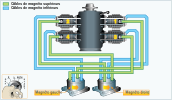
\includegraphics[width=0.5\textwidth]{01-EtudeAeronefs/img/systemesAvion/systemeAllumage.pdf}
  		\legende{Système d'allumage sur un moteur à 4 cylindres à plat)}{img:systemeAllumage}
	\end{figure}	
	
	\info{Le fait d'avoir 2 bougies permet aussi une meilleure combustion et donc que le moteur délivre toute sa puissance.}
	
	\info{Les moteurs à explosion d'avion léger sont généralement conçus pour être indépendants de toute source d'énergie extérieure. En particulier, une panne de l'alimentation électrique de bord n'aura pas d'impact sur la fonctionnement du moteur qui continuera à fonctionner normalement.}
	
	\subsubsection{Système d'alimentation en carburant}
	
 Pour fonctionner, un moteur à combustion interne nécessite d'être alimenté par un mélange d'air et d'essence dans un rapport d'environ $1/15^{ième}$ (quinze gramme d'air pour 1 gramme d'essence)\footnote{Le rapport exact est 14,7:1, soit 14,7~g d'air pour 1~g d'essence}. Ce rapport est nécessaire pour assurer un mélange st\oe chiométrique\footnote{Le mélange st\oe chiométrique pour un moteur à essence est le rapport idéal air/carburant qui brûle tout le carburant sans excès d'air.}, c'est-à-dire que la quantité d'oxygène admise dans le cylindre soit suffisante pour assurer la combustion complète du carburant qui l'accompagne. La combustion totale permet d'optimiser la consommation de carburant en extrayant le maximum d'énergie, mais également d'éviter un encrassement du moteur par la production de suies et autres dépôts qui accompagnent toujours une combustion incomplète.
	
	Dans un moteur, cette fonction peut être assurée par un carburateur ou un système d'injection. Sur beaucoup d'avions, on a encore recours assez largement aux carburateurs, bien que les systèmes d'injection tendent à se généraliser.
	
	\paragraph{Carburant utilisés}
	Les moteurs à explosion d'avion fonctionnent avec de l'essence. En fonction du moteur, on a recours à différentes qualités de carburant
	\begin{itemize}
		\item La 100LL, ou avgas \anglais{aviation gasoline}. Le LL est l'abréviation de \textit{low lead} (faiblement plombé). Ce carburant, spécialement conçu pour l'usage en aviation, contient du plomb, destiné à limiter le risque de cliquetis moteur. Les distributeurs de ce carburant garantissent également une faible présence d'eau contenue dans ce carburant. On peut identifier ce carburant à sa couleur bleue. Le plomb contenu dans ce carburant présente une toxicité.
		\item L'UL91, UL pour \textit{UnLeaded} (sans-plombe) est un carburant pour l'aviation, destiné à remplacer la 100LL, cependant, un moteur d'avion destiné à utiliser de la 100LL ne peut utiliser de l'UL91 sans modification. L'UL91 est de couleur rouge.
		\item Le sans plomb 98, l'essence automobile (appelé Mogas), est utilisé dans certains moteurs d'avion, notamment dans le monde ULM.
	\end{itemize}
	
	\paragraph{Le carburateur}
	
	Sur un carburateur, le papillon est commandé directement par la manette des gaz. Lorsque le papillon est fermé, la quantité de carburant aspiré est faible, ce qui réduit le régime de rotation du moteur. La pleine ouverte du papillon va au contraire permettre l'admission d'une grande quantité de mélange dans les cylindres.
	
	Le carburateur est notamment composé d'un tube venturi. Dans cette portion du carburateur, on réduit la section disponible pour le passage de l'air. Cela provoque, par effet Venturi, une accélération et une dépression, ce qui va permettre d'aspirer et de vaporiser le carburant présent au niveau du gicleur.
	
	\begin{figure}[H]
  		\centering
    		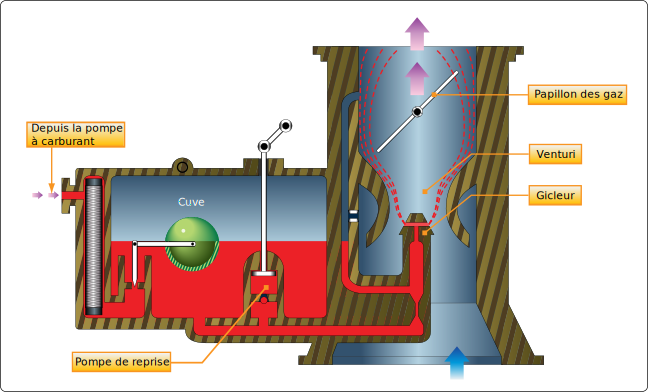
\includegraphics[width=0.9\textwidth]{01-EtudeAeronefs/img/systemesAvion/carburateur.pdf}
  		\legende{Schéma d'un carburateur}{img:carburateur}
	\end{figure}	
	
	Le carburateur dispose d'un petit réservoir appelé cuve, dans lequel le niveau de carburant, en provenance des réservoirs et mis en pression grâce à des pompes, est maintenu constant grâce à un flotteur qui commande l'ouverture d'un pointeau.
	
	Un dispositif appelé pompe de reprise, actionné mécaniquement lorsque la manette des gaz est avancée rapidement, permet d'envoyer dans le carburateur une quantité supplémentaire de carburant lorsque le pilote demande une augmentation rapide de la puissance. Cela permet d'aider le moteur à atteindre rapidement le régime demandé par le pilote.
	
	\subparagraph{Givrage carburateur}
	Au sein du carburateur, le tube Venturi est le siège d'une dépression. Comme toute baisse de pression, elle s'accompagne d'une baisse de la température. Cette baisse est suffisante pour atteindre le point de condensation puis de congélation de la vapeur d'eau présente dans l'air ou dans le carburant.
	
	Le carburateur peut alors subir un givrage : de la glace se forme dans le carburateur, ce qui va provoquer la réduction du passage disponible pour l'air. Cela peut aboutir, si rien n'est fait et que la situation est maintenue, à une réduction telle du passage de l'air que le moteur s'arrêtera.
	
	\begin{figure}[H]
  		\centering
    		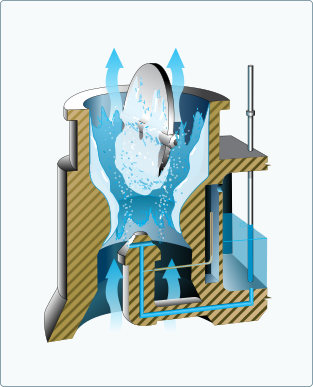
\includegraphics[width=0.25\textwidth]{01-EtudeAeronefs/img/systemesAvion/givrageCarbu.pdf}
  		\legende{Illustration d'un givrage carburateur}{img:givrageCarbu}
	\end{figure}
	
	Pour pallier ce risque, les moteurs à carburateurs sont généralement équipés de système de réchauffage du carburateur. On réchauffe de l'air en la faisant passer autour du pot d'échappement. L'air présenté en entrée du carburateur est ainsi suffisamment chaud pour que la chute de la température dans le carburateur ne présente plus de risque d'atteinte du point de congélation.
	
	\begin{figure}[H]
  		\centering
    		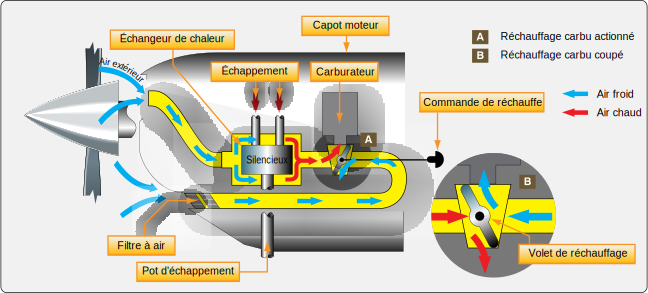
\includegraphics[width=0.85\textwidth]{01-EtudeAeronefs/img/rechauffeCarbu.pdf}
  		\legende{Fonctionnement du réchauffage carburateur}{img:rechauffeCarbu}
	\end{figure}
	
	Ce réchauffage du carburateur n'est cependant utilisé que lorsqu'il est strictement nécessaire car l'air plus chaud étant moins dense, l'usage du réchauffage carburateur provoque une réduction de la puissance délivrée par le moteur. 
	
	En effet, l'air chaud étant moins dense, la quantité d'oxygène disponible pour la combustion s'en trouve réduite. Il en résulte un enrichissement du mélange (trop de carburant par rapport à l'oxygène disponible dans l'air admis), qui est alors trop riche pour permettre au moteur de délivrer sa pleine puissance. Par ailleurs, l'usage de la réchauffe carbu à pleine puissance augmente notablement le risque de détonation 
	
	%TODO : ajouter un texte (et l'image ?) pour expliciter pourquoi le réchauffage carbu n'esst généralement pas utilisé à pleine puissance
	
	\info{L'air utilisé quand on active le réchauffage carburateur n'est pas filtré, contrairement à l'air froid. Il est donc déconseillé d'utiliser le réchauffage carburateur au sol, car cela augmente le risque que des contaminants soient ingérés par le moteur.}
	
	
	\subsection{Motorisation électrique}

	
	\subsection{Hélices et moteurs}
	
	\subsection{Propulseurs à réaction}
		\subsubsection{Turboréacteurs}
		Le turboréacteur \anglais{turbojet} est un système de propulsion qui produit une poussée grâce à l'accélération d'un flux d'air entre l'entrée et la sortie du réacteur.
		
		Un réacteur simple est composé :
		\begin{itemize}
			\item d'une entrée d'air \anglais{air inlet}
			\item d'un compresseur \anglais{compressor} dont le rôle est de comprimer l'air qui rentre dans le réacteur
			\item d'une chambre de combustion \anglais{combustion chamber} dans lequel le carburant est injecté pour être brûlé
			\item d'une turbine \anglais{turbine} dont le rôle est de récupérer une partie de l'énergie produite par la combustion
			\item d'une tuyère \anglais{nozzle}, dont le rôle est de canaliser les gaz de combustion, et d'optimiser la poussée.
		\end{itemize}
		\begin{figure}[H]
  		\centering
    		\includegraphics[width=0.75\textwidth]{01-EtudeAeronefs/img/turbomachines/turboreacteur-schema.pdf}
  		\legende{Schéma de fonctionnement d'un turboréacteur}{img:turboreacteur-schema}
		\end{figure}		
		
		L'air admis dans le réacteur est d'abord comprimé par le compresseur, ce qui augmente sa pression et sa température. Le carburant, injecté dans la chambre de combustion, s'enflamme alors spontanément, ce qui provoque une augmentation du volume, de la température et de la vitesse des gaz au sein du réacteur. Ces gaz, éjectés vers l'arrière passent alors au travers de la turbine. Celle ci prélève une partie de l'énergie de gaz pour permettre l'entraînement, via un arbre de transmission, du compresseur à l'entrée du réacteur. Enfin, les gaz sont éjectés à haute vitesse par la tuyère, ce qui produit la poussée qui propulse l'aéronef.
		
		Les réacteurs utilisent généralement comme carburant du kérosène, dit Jet A1. %TODO voir si on parle ici de l'intrêt du JetA1 pour l'aviation : sécurité par haut point éclair, point de congélation bas...
		
		\paragraph{Réacteur simple flux}
		Le réacteur simple flux est la version la plus simple du turboréacteur. Dans cette configuration, l'ensemble du flux d'air traverse la chambre de combustion et l'ensemble du réacteur.
		\begin{figure}[H]
  		\centering
    		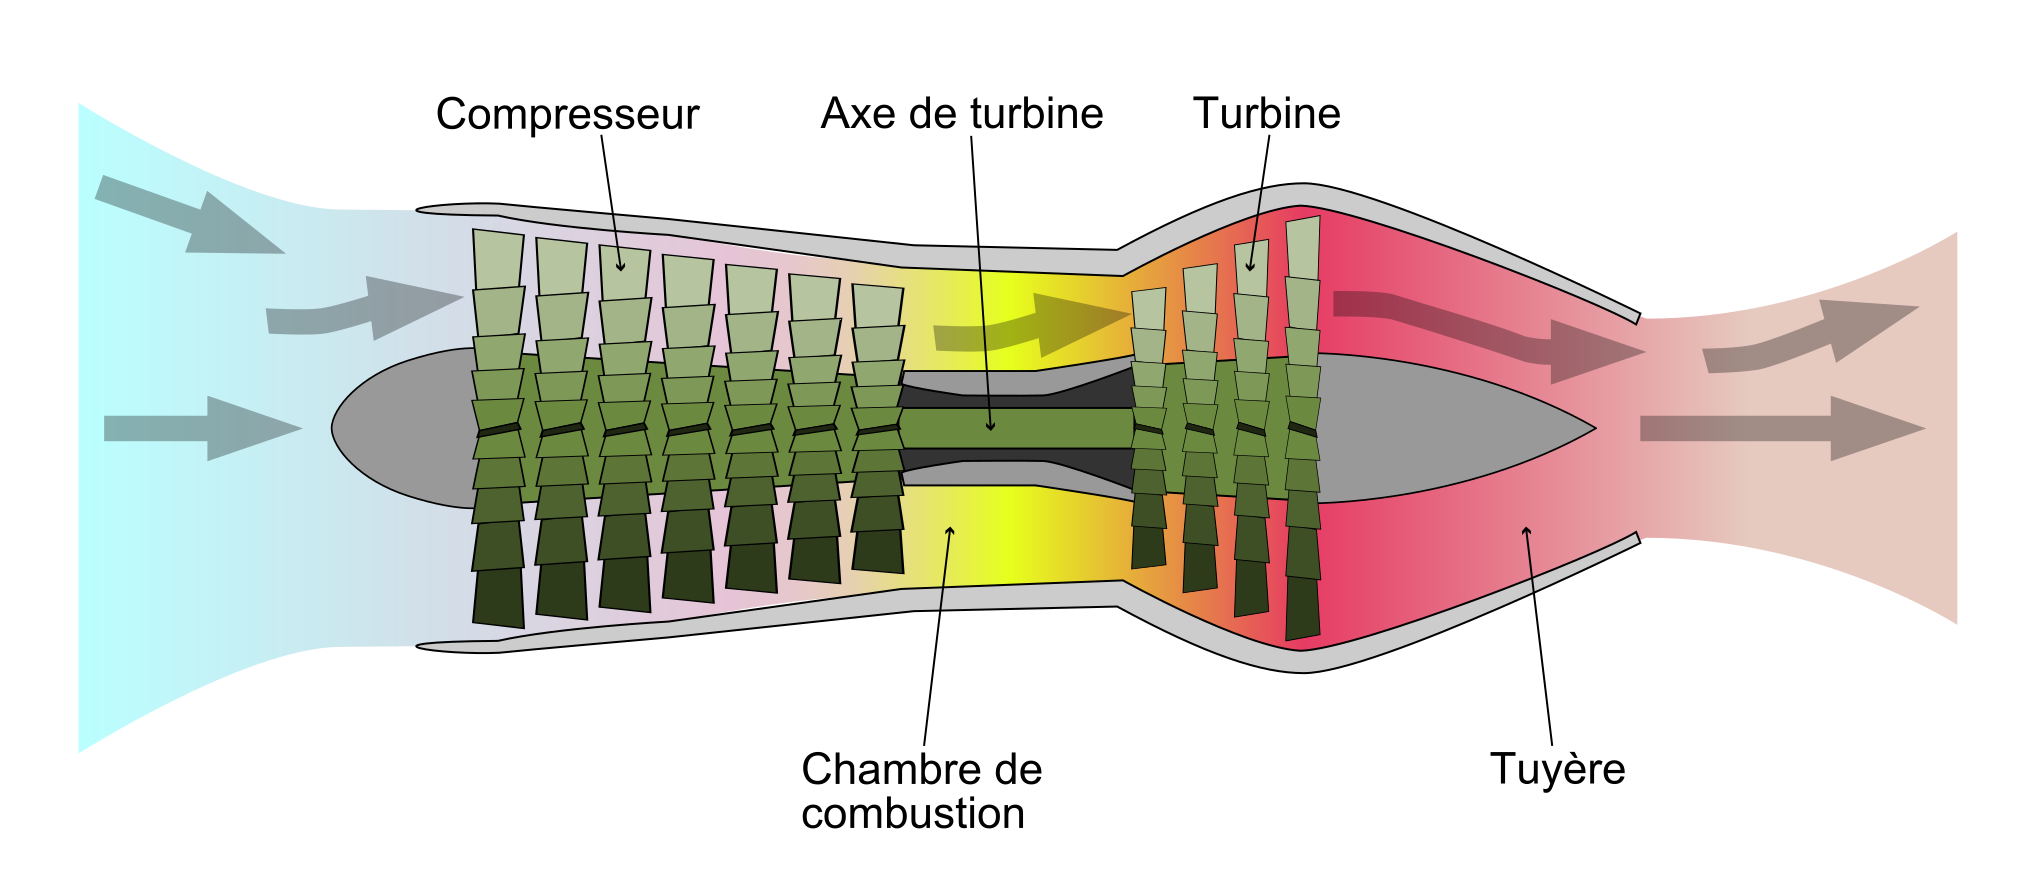
\includegraphics[width=0.75\textwidth]{01-EtudeAeronefs/img/turbomachines/turboreacteur-simpleFlux.pdf}
  		\legende{Schéma d'un turboréacteur simple corps simple flux}{img:turboreacteur-simpleFlux}
		\end{figure}	
		
		Ce type de réacteur est simple mais très bruyant, et sa consommation de carburant est élevée.
		\paragraph{Réacteur double corps}
		Pour augmenter l'efficacité des réacteurs, les ingénieurs ont souhaité augmenter le taux de compression dans le réacteur. Pour cela, ils ont ajouté un ensemble compresseur-turbine. Ainsi, le réacteur double corps est composé :
		\begin{itemize}
			\item d'un compresseur dit basse pression, 
			\item suivi d'un compresseur haute pression,
			\item de la chambre de combustion,
			\item d'une turbine haute pression,
			\item d'une turbine basse pression.
		\end{itemize}	
		Les axes des 2 ensembles compresseur-turbine sont concentriques : l'axe basse pression passe dans l'axe haute pression.
	
		\paragraph{Réacteur double flux}
		Dans un réacteur double flux \anglais{turbofan}, on sépare le flux d'air entrant en 2 parties :
		\begin{itemize}
			\item le flux primaire qui traverse le réacteur,
			\item le flux secondaire, qui contourne le réacteur.
		\end{itemize}
		Dans ce type de réacteur, le flux secondaire est mis en mouvement par une grande hélice carénée à l'avant du réacteur : la soufflante \anglais{fan}, elle même entraînée via l'arbre de turbine.	
		
		\begin{figure}[H]
  		\centering
    		\includegraphics[width=0.75\textwidth]{01-EtudeAeronefs/img/turbomachines/turboreacteur-doubleFlux.pdf}
  		\legende{Schéma d'un turboréacteur double corps double flux}{img:turboreacteur-doubleFlux}
		\end{figure}	
		
		Dans un réacteur double flux, la majorité de la poussée (environ 80~\%) est produite par le flux secondaire.
		
		Ce type de réacteur est bien plus économique en carburant qu'un simple flux et est bien plus silencieux.
		
		Un réacteur double flux est toujours composé d'un réacteur double corps, car la soufflante est entraînée par l'axe du compresseur basse pression.
		
		\subparagraph{Taux de dilution}
		Le rapport entre le flux d'air primaire et le flux d'air secondaire est appelé taux de dilution. 
		
		Les réacteurs les plus modernes peuvent atteindre un rapport de 10 pour 1, ce qui signifie que la quantité d'air qui passe autour du réacteur est 10 fois supérieure à celle qui passe dans la turbine. 
		
		\info{Ce type de réacteur à fort taux de dilution, utilisé sur A350 ou B777X peut ainsi aspirer 1.5 tonnes d'air par seconde.}
		
		\paragraph{Postcombustion}
		La postcombustion \anglais{afterburner} ou réchauffe, est une technique utilisée pour augmenter la poussée d'un réacteur. Cette augmentation de poussée est obtenue par l'injection de carburant dans la tuyère, ce qui réenflamme les gaz à la sortie du réacteur.
		
		\begin{figure}[H]
  		\centering
    		\includegraphics[width=0.45\textwidth]{01-EtudeAeronefs/img/postcombustion-FA-18.jpg}
  		\legende{F/A-18 au catapultage avec postcombustion allumée}{img:postcombustion-FA-18}
		\end{figure}	
		
		\info{La postcombustion est essentiellement utilisée sur les avions de combat. Les seuls avions civils qui ont utilisé la postcombustion sont les avions de ligne supersoniques Concorde et son homologue soviétique le Tupolev Tu144.\\ Sur Concorde, l'augmentation de poussée était de l'ordre de 25~\%, soit l'équivalent d'un cinquième réacteur. Elle était utilisée au décollage et lors de l'accélération vers la croisière supersonique. La consommation avec la postcombustion allumée était de 80~tonnes par heure, contre 15 à 20~tonnes par heure en croisière supersonique}
		
		\subsubsection{Statoréacteurs}
		Le statoréacteur \anglais{ramjet} est un système de propulsion qui produit sa poussée grâce à la combustion du kérosène dans un tube sans aucune pièce mobile (d'où le préfixe \textit{stato}). Sans aucune pièce mobile, c'est le propulseur le plus simple.
		\begin{figure}[H]
  		\centering
    		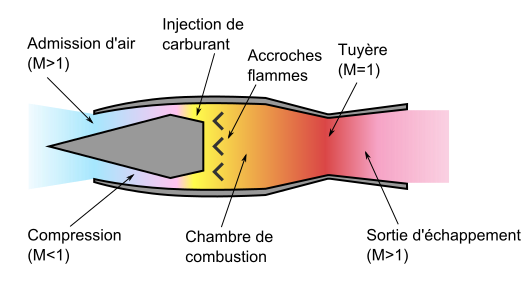
\includegraphics[width=0.75\textwidth]{01-EtudeAeronefs/img/statoreacteur.pdf}
  		\legende{Schéma d'un statoréacteur}{img:statoreacteur}
		\end{figure}	
		
		Cependant, cette simplicité a un cout : pour que l'air puisse être comprimé sans aucune pièce mobile, on ne peut se reposer que sur la géométrie du statoréacteur, et sur la vitesse de l'air en entrée du propulseur. Cela implique que le statoréacteur ne fonctionne pas à vitesse faible pour nulle. Les aéronefs propulsés par des statoréacteurs doivent donc disposer d'un autre mode de propulsion pour assurer leur décollage et leur accélération, soit être largués par un autre aéronef porteur qui assurera pour eux le décollage et l'accélération.
		
		\histoire{Le statoréacteur est conceptualisé dès l'année 1913 par l'ingénieur français  René Lorin. Le \textit{Leduc 010}, conçu par l'ingénieur français René Leduc, deviendra en 1949 le premier aéronef propulsé par un statoréacteur.}
	
		\subsubsection{Moteurs fusées}
		Les moteurs fusées sont conçus pour pouvoir fonctionner en dehors de l'atmosphère terrestre, dans un environnement sans oxygène, donc sans comburant. Le comburant étant indispensable à la combustion, les moteurs fusée disposent, en plus de la traditionnelle arrivée de carburant, d'une alimentation en comburant en provenance des réservoirs du vaisseau sur lequel ils sont installés.
		
		\begin{figure}[H]
  		\centering
    		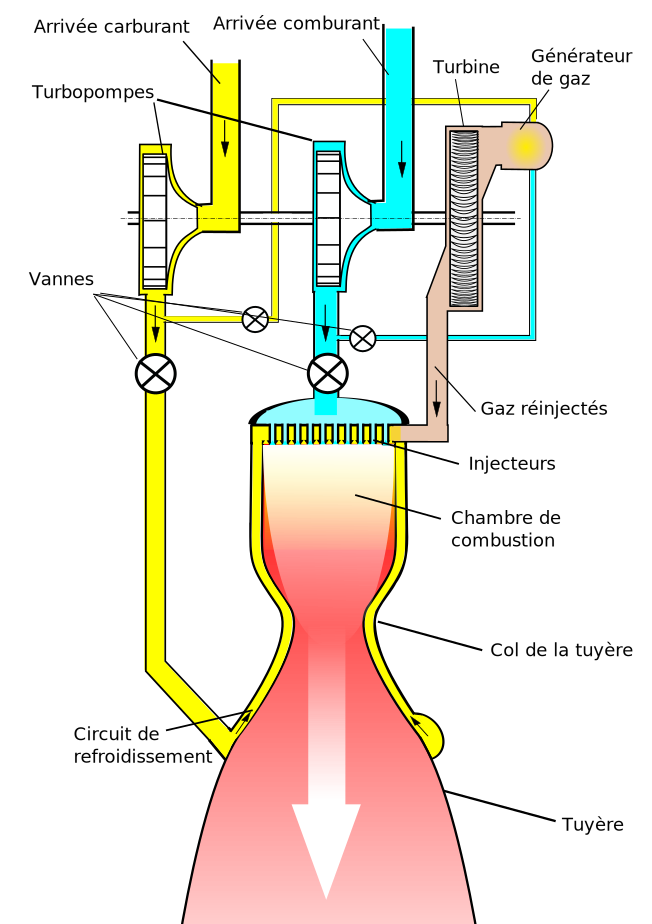
\includegraphics[width=0.65\textwidth]{01-EtudeAeronefs/img/moteurFusee.pdf}
  		\legende{Schéma d'un moteur fusée à propergols liquides}{img:moteurFusee}
		\end{figure}	
		
	\subsection{Turbopropulseurs et turbomoteurs}
	Le turbopropulseur \anglais{turboprop} est un turboréacteur dont on récupère la majeure partie de la puissance sur l'arbre de la turbine pour la transmettre à une hélice. Compte tenu de la vitesse de rotation de l'arbre d'une turbine, il est nécessaire de réduire la vitesse de rotation via un réducteur avant de la transmettre à l'hélice.
	
		\begin{figure}[H]
  		\centering
    		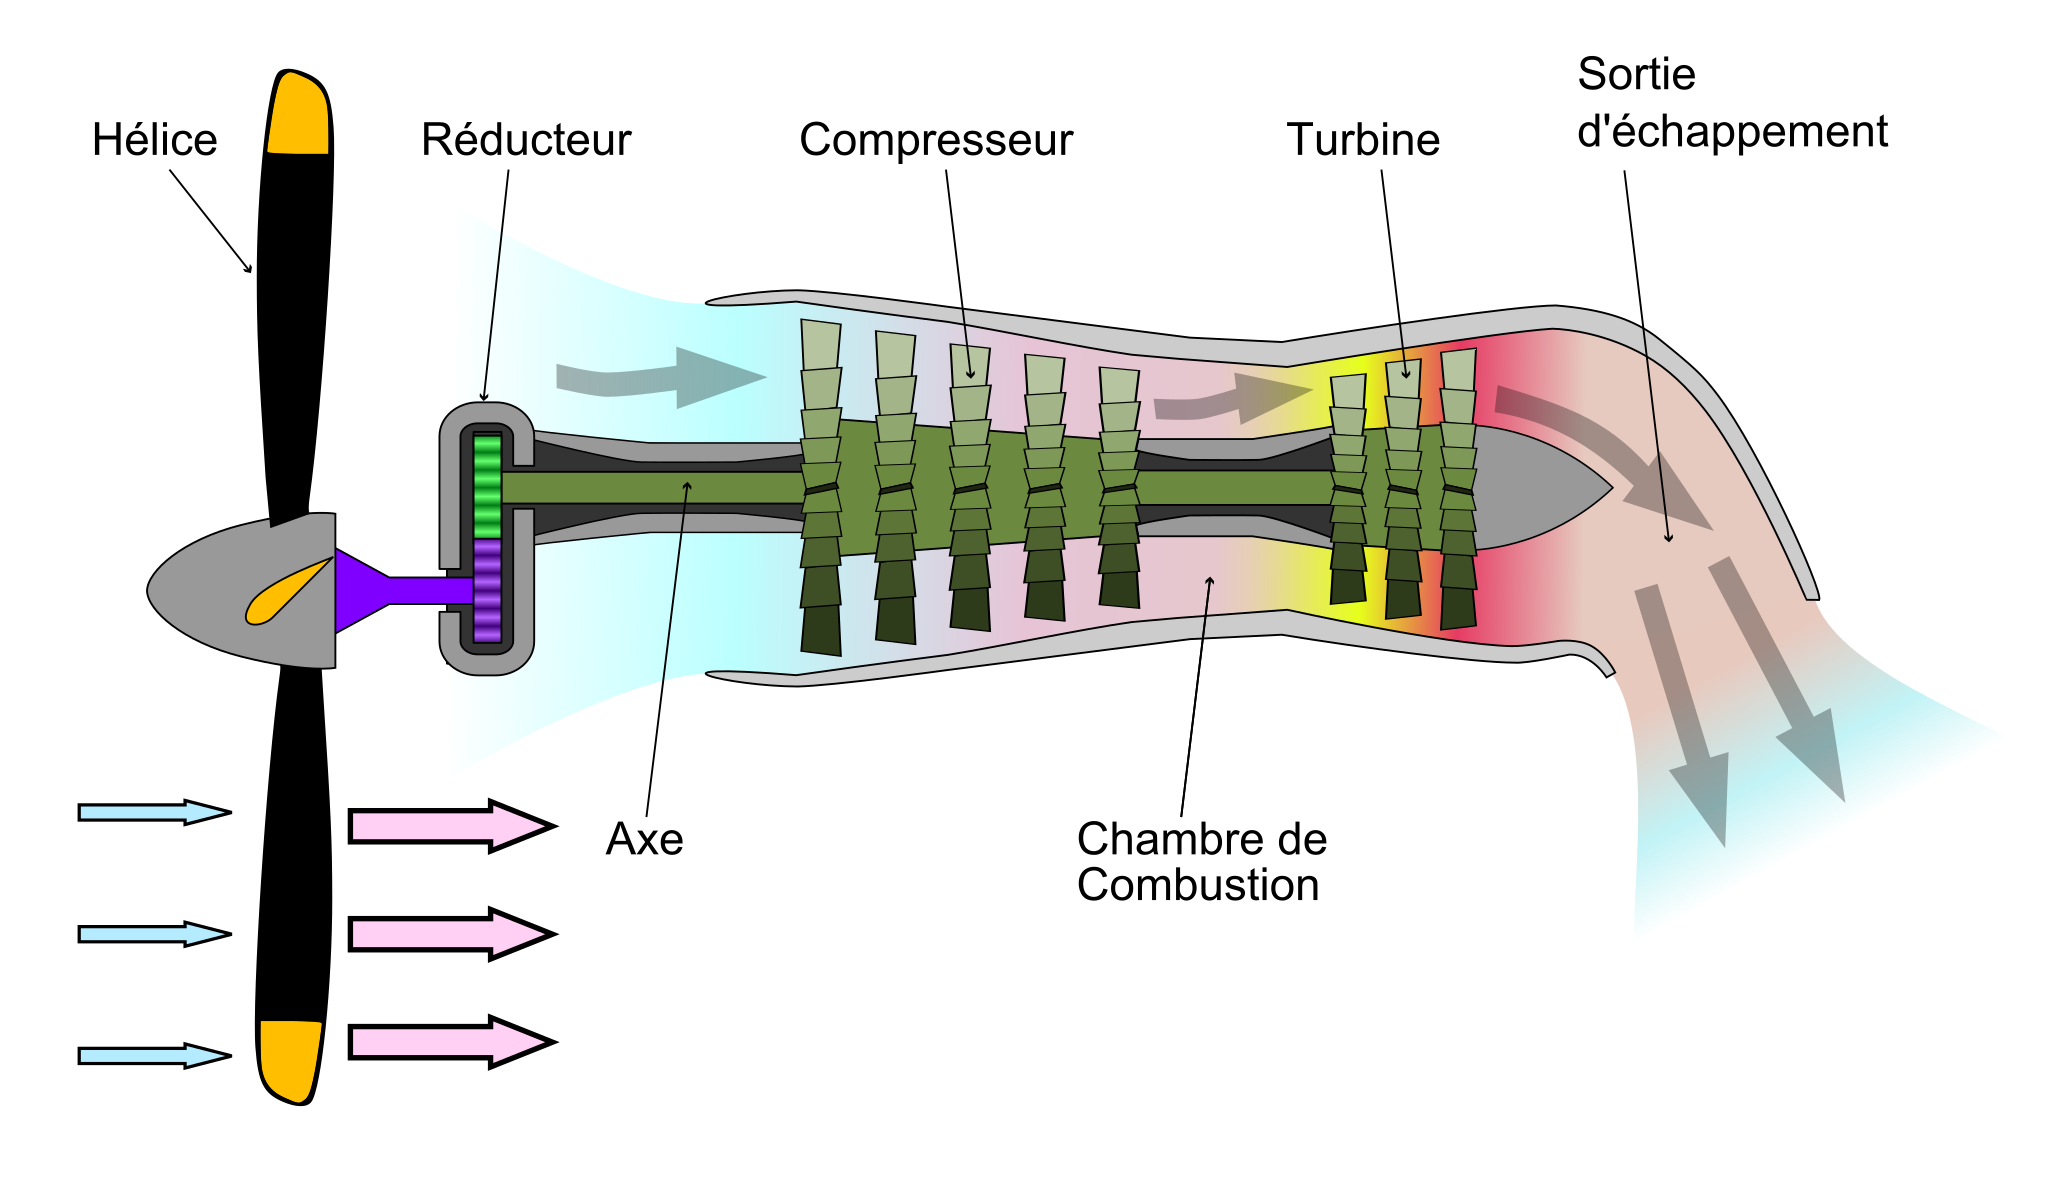
\includegraphics[width=0.75\textwidth]{01-EtudeAeronefs/img/turbomachines/turbopropulseur.pdf}
  		\legende{Schéma d'un turbopropulseur}{img:turbopropulseur}
		\end{figure}	
		
		Les turbopropulseurs sont utilisés notamment sur les avions de ligne destinés aux liaison de courte distance.
		
		Par rapport à un moteur à explosion, utiliser une turbine pour entraîner une hélice présente de nombreux avantages :
		\begin{itemize}
			\item efficacité : un turbopropulseur a un meilleur rendement qu'un moteur à explosion
			\item fiabilité : les turbomachines sont très fiables. Cela permet d'augmenter les périodicités d'entretien et la fiabilité est un paramètre important d'un usage aéronautique\footnote{Par exemple, le turbine PT6 dispose d'un taux d'arrêt en vol de 1 pour 300 000 heures, ce qui est exceptionnel}
			\item utilisation de kérosène, carburant aisément disponible partout dans le monde et qui présente des caractéristiques qui le rendent très sûr (carburant difficilement inflammable).
		\end{itemize}
	
		
	\subsection{Contraintes liées au développement durable}
